
%(BEGIN_QUESTION)
% Copyright 2012, Tony R. Kuphaldt, released under the Creative Commons Attribution License (v 1.0)
% This means you may do almost anything with this work of mine, so long as you give me proper credit

En trefase nedtransformator leverer 480 VAC til to resistive laster. Sekundærviklingen er ``corner-grounded'' på X2-ben:

$$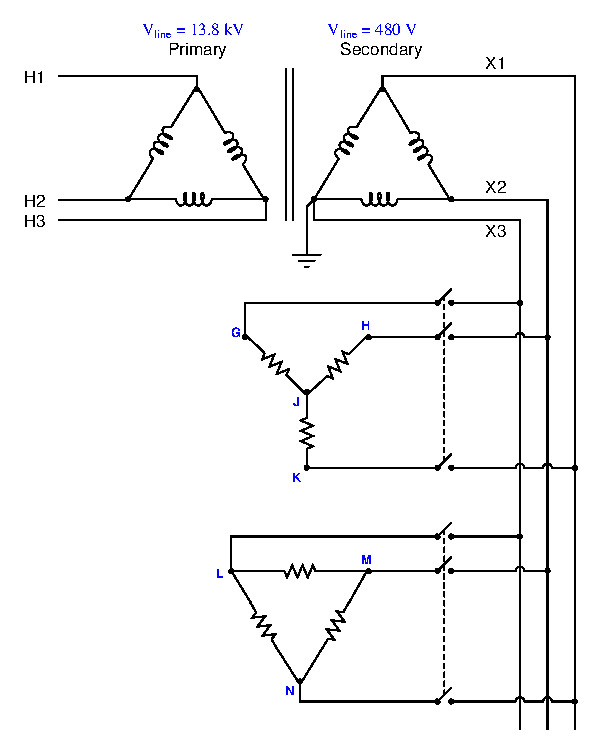
\includegraphics[width=15.5cm]{i00966x01.eps}$$

Bestem fase-til-jord-spenningene når begge laster er innkoblet:

\begin{itemize}
\item{} $V_{G}$ = \underbar{\hskip 50pt} volt
\vskip 10pt
\item{} $V_{H}$ = \underbar{\hskip 50pt} volt
\vskip 10pt
\item{} $V_{J}$ = \underbar{\hskip 50pt} volt
\vskip 10pt
\item{} $V_{K}$ = \underbar{\hskip 50pt} volt
\vskip 10pt
\item{} $V_{L}$ = \underbar{\hskip 50pt} volt
\vskip 10pt
\item{} $V_{M}$ = \underbar{\hskip 50pt} volt
\vskip 10pt
\item{} $V_{N}$ = \underbar{\hskip 50pt} volt
\end{itemize}

Anta øvre last 8.4 kW og nedre last 3.9 kW. Beregn strømmen i linje H2.

\underbar{file i00966}
%(END_QUESTION)





%(BEGIN_ANSWER)

\begin{itemize}
\item{} $V_{G}$ = 0 volt
\vskip 10pt
\item{} $V_{H}$ = 480 volt
\vskip 10pt
\item{} $V_{J}$ = 277.13 volt
\vskip 10pt
\item{} $V_{K}$ = 480 volt
\vskip 10pt
\item{} $V_{L}$ = 0 volt
\vskip 10pt
\item{} $V_{M}$ = 480 volt
\vskip 10pt
\item{} $V_{N}$ = 480 volt
\end{itemize}

Total effekt er 12.3 kW. Linjestrøm på primærsiden (uten tap):

$$I_{line} = {12300 \over \sqrt{3} (13800)} = 0.5146 \hbox{ A}$$

%(END_ANSWER)





%(BEGIN_NOTES)


%INDEX% Electronics review: 3-phase voltage/current/power calculation

%(END_NOTES)

